\documentclass{article}
\usepackage{fullpage}

\usepackage{graphicx} % For including graphics
\usepackage{subcaption} % For subfigures
\usepackage{tikz}
\usepackage{amsmath}
\usepackage{pgfplots}
\pgfplotsset{compat=1.17}
\usepackage{tikz,tikz-3dplot}
\tdplotsetmaincoords{80}{45}
\tdplotsetrotatedcoords{-90}{180}{-90}


% CONE PLOTTING
%% style for surfaces
\tikzset{surface/.style={draw=gray!70!black, fill=gray!40!white, fill opacity=.6}}

%% macros to draw back and front of cones
%% optional first argument is styling; others are z, radius, side offset (in degrees)
\newcommand{\coneback}[4][]{
  %% start at the correct point on the circle, draw the arc, then draw to the origin of the diagram, then close the path
  \draw[canvas is xy plane at z=#2, #1] (45-#4:#3) arc (45-#4:225+#4:#3) -- (O) --cycle;
}
\newcommand{\conefront}[4][]{
  \draw[canvas is xy plane at z=#2, #1] (45-#4:#3) arc (45-#4:-135+#4:#3) -- (O) --cycle;
}

\begin{document}

\begin{figure}
     \begin{subfigure}[b]{0.325\textwidth}
          \centering
          \resizebox{0.8 \linewidth}{!}{
              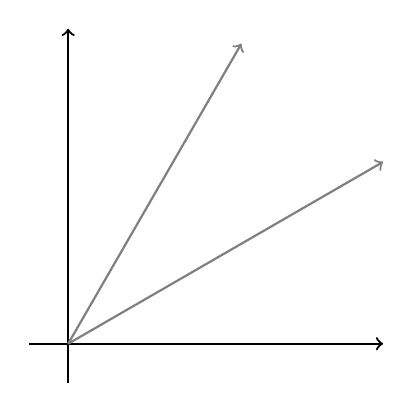
\begin{tikzpicture}
      		\draw[->,thick] (-0.5,0) -- (4,0);
      		\draw[->,thick] (0,-0.5) -- (0,4);
      		\draw[gray,thick,->,domain=0:4] plot (\x,{\x/sqrt(3)});
      		\draw[gray,thick,->,domain=0:2.2] plot (\x,{sqrt(3)*\x});
    	    \end{tikzpicture}         
          }  
          \caption*{Caption A}
          \label{fig:A}
     \end{subfigure}
     \begin{subfigure}[b]{0.325\textwidth}
          \centering
          \resizebox{0.8 \linewidth}{!}{
              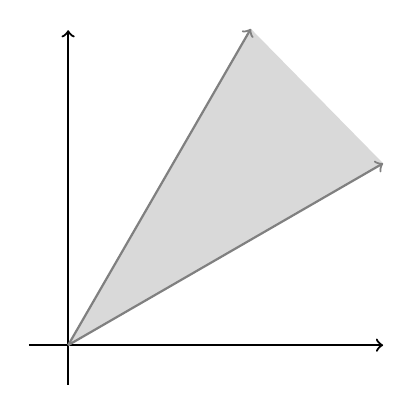
\begin{tikzpicture}
      		\draw[->,thick] (-0.5,0) -- (4,0);
      		\draw[->,thick] (0,-0.5) -- (0,4);
		    \fill[gray!30] (0,0) -- plot[domain=0:4] (\x,{\x/sqrt(3)}) -- plot[domain=2.32:0] (\x,{sqrt(3)*\x}) -- cycle;
      		\draw[gray,thick,->,domain=0:4] plot (\x,{\x/sqrt(3)});
      		\draw[gray,thick,->,domain=0:2.32] plot (\x,{sqrt(3)*\x});
    	\end{tikzpicture}          
          }  
          \caption*{Caption B}
          \label{fig:B}
     \end{subfigure}
     \begin{subfigure}[b]{0.325\textwidth}
          \centering
          \resizebox{\linewidth}{!}{
              \begin{tikzpicture}[tdplot_main_coords]
				\coordinate (O) at (0,0,1);
         		 \draw (0,0,-1) -- (O);
      			 \draw[->] (-5,0,1) -- (5,0,1) node[right] {};
     		 	 \draw[->] (0,-5,1) -- (0,5,1) node[right] {};
     		     \coneback[surface]{3}{2}{11}
     		     \draw[->] (O) -- (0,0,5) node[above] {};
      		     \conefront[surface]{3}{2}{11}
   	 \end{tikzpicture}
          }  
          \caption*{Caption C}
          \label{fig:C}
     \end{subfigure}
 \end{figure}
 
\end{document}
